%% Standalone source of one report figure. Rebuild: pdflatex -output-directory=.. fig-07-segmenter.tex
\documentclass[11pt]{standalone}
\usepackage[T1]{fontenc}
\usepackage[utf8]{inputenc}
\usepackage{lmodern}
\usepackage{microtype}
\usepackage{amsmath,amssymb}
\usepackage{xcolor}
\usepackage{tikz}
\usetikzlibrary{arrows.meta,positioning,shapes.geometric,fit,calc,backgrounds}
\usepackage{pgfplots}
\usepackage{pgfplotstable}
\pgfplotsset{compat=1.18}
\setlength{\textwidth}{472.31595pt}  %% = the report's text width, so widths given in \textwidth match
\definecolor{gmblue}{HTML}{0B3D6E}
\definecolor{gmok}{HTML}{1E7B34}
\definecolor{gmwarn}{HTML}{B35C00}
\definecolor{gmbad}{HTML}{A32020}
\definecolor{gmgrey}{HTML}{5A5F66}
\definecolor{gmlight}{HTML}{EEF3F8}
\definecolor{gmteal}{HTML}{1B7A8C}
\newcommand{\done}{\textcolor{gmok}{\textbf{Done}}}
\newcommand{\partly}{\textcolor{gmwarn}{\textbf{Partly}}}
\newcommand{\pending}{\textcolor{gmbad}{\textbf{Pending}}}
\newcommand{\pass}{\textcolor{gmok}{\textbf{PASS}}}
\newcommand{\fail}{\textcolor{gmbad}{\textbf{FAIL}}}
\newcommand{\code}[1]{\texttt{\small #1}}
\newcommand{\INR}{INR~}
\newcommand{\gbar}[5]{\fill[#5] (#1,-#3+0.32) rectangle (#2,-#3-0.32);
  \node[anchor=east,font=\scriptsize] at (-0.3,-#3) {#4};}

\tikzset{
  box/.style={draw=gmblue, rounded corners=3pt, fill=gmlight, align=center, font=\small, inner sep=5pt,
              minimum height=9mm},
  gstep/.style={draw=gmblue, rounded corners=3pt, fill=white, align=center, font=\footnotesize, inner sep=4pt,
               text width=27mm, minimum height=11mm},
  st/.style={draw=gmblue, rounded corners=6pt, fill=gmlight, font=\scriptsize\ttfamily, inner sep=3pt,
             minimum height=6mm},
  arr/.style={-{Stealth[length=2.2mm]}, thick, gmblue},
  darr/.style={-{Stealth[length=2mm]}, gmgrey, dashed},
}

\begin{document}
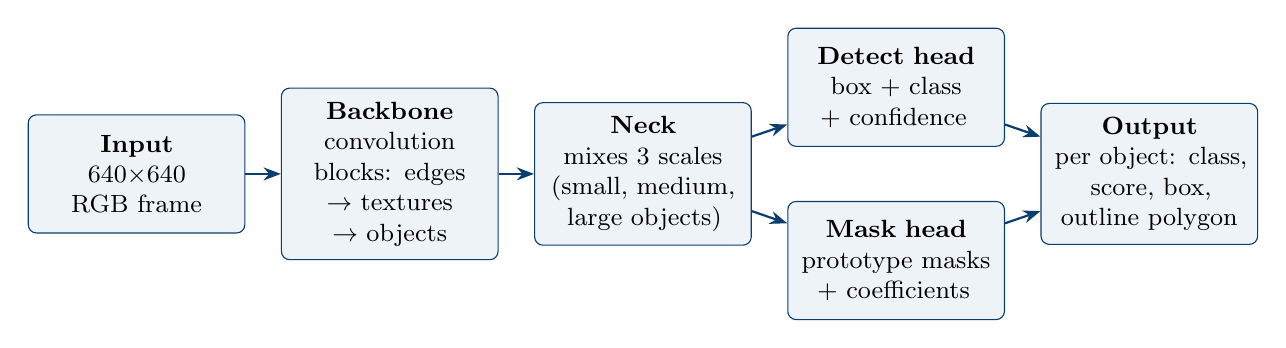
\begin{tikzpicture}[node distance=4.5mm, every node/.style={box, text width=24mm, minimum height=15mm}]
  \node (in) {\textbf{Input}\\640$\times$640\\RGB frame};
  \node[right=of in] (bb) {\textbf{Backbone}\\convolution\\blocks: edges\\$\rightarrow$ textures\\$\rightarrow$ objects};
  \node[right=of bb] (nk) {\textbf{Neck}\\mixes 3 scales\\(small, medium,\\large objects)};
  \node[right=of nk, yshift=11mm] (dh) {\textbf{Detect head}\\box + class\\+ confidence};
  \node[right=of nk, yshift=-11mm] (mh) {\textbf{Mask head}\\prototype masks\\+ coefficients};
  \node[right=of dh, yshift=-11mm] (out) {\textbf{Output}\\per object: class,\\score, box,\\outline polygon};
  \draw[arr] (in)--(bb); \draw[arr] (bb)--(nk); \draw[arr] (nk)--(dh); \draw[arr] (nk)--(mh);
  \draw[arr] (dh)--(out); \draw[arr] (mh)--(out);
\end{tikzpicture}
\end{document}
